\section{Mechanical Models II}
\label{MechModelsII:sec}

\subsection{Units}

\subsection{Multi-point springs}

OPTIONAL

\subsubsection{Operation}

\subsubsection{Example: A single multi-point spring}

%\begin{figure}[h]
%\begin{center}
%\iflatexml
% 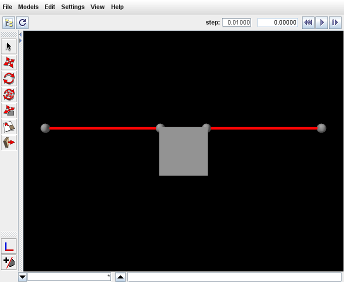
\includegraphics[]{images/MultiPointSpring}
%\else
% 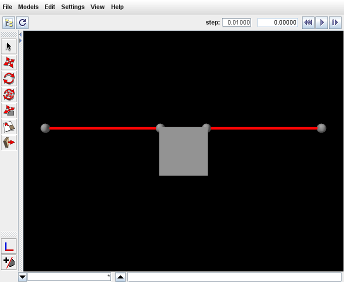
\includegraphics[width=3.75in]{images/MultiPointSpring}
%\fi
%\end{center}
%\caption{MultiPointSpring model loaded into ArtiSynth.}
%\label{MultiPointSpring:fig}
%\end{figure}
%
%A simple model showing a multi-point spring is defined in
%%
%\begin{verbatim}
%  artisynth.demos.tutorial.MultiPointSpring
%\end{verbatim}
%

% MultiPointSpring

\subsection{Point-to-point muscles}
\label{PointToPointMuscles:sec}

\subsubsection{Muscle materials}

\subsubsection{Example: Muscle attached to a rigid body}

\begin{figure}[h]
\begin{center}
\iflatexml
 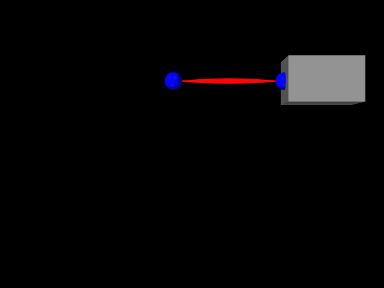
\includegraphics[]{images/SimpleMuscle}
\else
 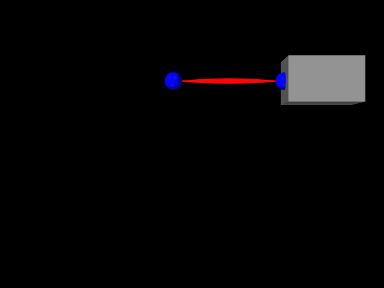
\includegraphics[width=3.75in]{images/SimpleMuscle}
\fi
\end{center}
\caption{SimpleMuscle model loaded into ArtiSynth.}
\label{SimpleMuscle:fig}
\end{figure}

A simple model showing a single muscle connected to a rigid
body is defined in
%
\begin{verbatim}
  artisynth.demos.tutorial.SimpleMuscle
\end{verbatim}
%

% SimpleMuscle

\subsubsection{Multi-point muscles}

\subsection{Mesh components}

OPTIONAL 

\subsubsection{Fixed meshes}

\subsubsection{Simple mesh example}

% SimpleMesh

\subsubsection{Skinned meshes}

\subsubsection{Simple skinned mesh example}

% SimpleSkinnedMesh

\subsection{Collision Handling}

\subsubsection{Collidable bodies}

\subsubsection{Enabling collisions in code}

\subsubsection{Example: Collision with a plane}

\begin{figure}[h]
\begin{center}
\iflatexml
 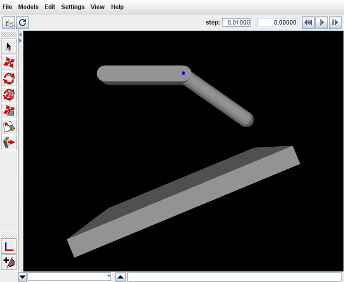
\includegraphics[]{images/JointedCollide}
\else
 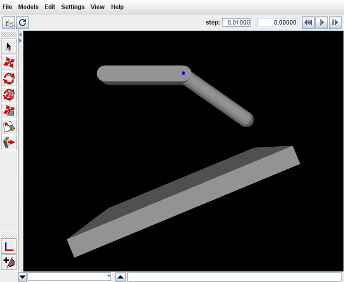
\includegraphics[width=3.75in]{images/JointedCollide}
\fi
\end{center}
\caption{JointedCollide model loaded into ArtiSynth.}
\label{JointedCollide:fig}
\end{figure}

A simple model illustrating collision between two jointed rigid bodies
and a plane is defined in
%
\begin{verbatim}
  artisynth.demos.tutorial.JointedCollide
\end{verbatim}
%

% JointedCollide

\subsubsection{implementation and limitations}

%\subsection{Moving non-dynamic components}

\subsection{General component arrangements}
\label{GeneralArrangements:sec}

OPTIONAL

\subsubsection{Component lists}

\subsubsection{General arrangement example}

% NetDemo

\subsubsection{Legacy containers in MechModel}

\subsection{Render properties}
\label{RenderProperties:sec}

\subsubsection{Render property taxonomy}

\subsubsection{Setting render properties}

\subsection{Scaling and transforming}

OPTIONAL

\subsubsection{The ScalableUnits interface}

\subsubsection{The TransformableGeometry interface}
